

\section{Basic \tc Protocol}
\label{sec:protocols}
We now describe the operation of \tc at the protocol level. The basic protocol is conceptually simple: a user contract \reqcont requests a datagram from the \tcontract \tcont, \tcont forwards the request to \engine and then returns the response to \reqcont. There are many details, however, relating to message contents and protection and the need to connect the off-chain parts of \tc with the blockchain.

First we give a brief protocol overview. Then we enumerate the data flows in \tc. Finally, we provide a component-level view of the protocol by specifying the operation of the \tcontract, \medname, and \encname. We present these  as ideal functionalities, inspired by the universal-composability (UC) framework, in order to abstract away implementation details and as a springboard for formal proofs of security. We omit details in this section on how payment is incorporated into \tc, deferring this delicate aspect of the system design to Section~\ref{sec:enhanced_protocol}.

\subsection{Datagram Lifecycle}

The lifecycle of a datagram may be briefly summarized in the following steps:

\vspace{-2mm}
\begin{itemize}
  \setlength{\itemsep}{2pt}
  \setlength{\parskip}{0pt}
  \setlength{\parsep}{0pt}
\item {\bf Initiate request.} \reqcont sends a datagram request to \tcont on the blockchain.

\item {\bf Monitor and relay.} The \medname monitors \tcont and relays any incoming datagram request with parameters \dgform to the \encname.

\item {\bf Securely fetch feed.} To process the request specified in \dgform, the \encname contacts a data source via HTTPS and obtains the requested datagram. It forwards the datagram via the Relay to \tcont.

\item {\bf Return datagram.} \tcont returns the datagram to \reqcont.
\end{itemize}
\vspace{-2mm}

\noindent We now make this data flow more precise. 

\subsection{Data Flows}
\label{sec:protocol-data-flows}

A datagram request by \reqcont takes the form of a message $m_1 = (\dgform, \dgcallback)$ to \tcont on the blockchain. $\dgform$ specifies the requested datagram, e.g.~${\sf params} := (\weburl, {\sf spec}, T)$, where $\weburl$ is the target data source, {\sf spec} specifies content of a the datagram to be retrieved (e.g., a stock ticker at a particular time), and $T$ specifies the delivery time for the datagram (initiated by scraping of the data source). The parameter $\dgcallback$ in $m_1$ indicates the entry point in \reqcont to which the datagram is to be returned. (In principle, $\dgcallback$ could point to a different contract, but \tc does not yet adopt this generalization.) 

\tcont generates a fresh unique $\dgid$ and forwards $m_2 = (\dgid, \dgform)$ to the \encname. It receives in return a return message $m_3 = (\dgid, \dgform, \dgm)$ from the \tc service, where $\dgm$ is the datagram (e.g.~the desired stock ticker price). \tcont checks the consistency of $\dgform$ on the incoming and outgoing messages, and if they match forwards $\dgm$ to the entry point \dgcallback in \reqcont in message $m_4$.

For simplicity here, we assume that $\reqcont$ makes a one-time datagram request. Thus it can trivially match $m_4$ with $m_1$. Our full protocol contains an optimization by which $\tcont$ returns $\dgid$ to $\reqcont$ after $m_1$ as a consistent, trustworthy identifier for all data flows. This enables straightforward handling of multiple datagram requests from the same instance of $\reqcont$.

Fig.~\ref{fig:dataflow} shows the data flows involved in processing a datagram request. For simplicity, the figure omits the \medname, which is only responsible for data passing.


%\begin{figure}[h!]
%\centering
%\begin{tikzpicture}
%  [entity/.style={rectangle,draw=black,minimum height=3em,text width=6em,align=center},
%   trusted/.style={fill=green!30},
%   communication/.style={blue,ultra thick,text=black},
%   bg-box/.style={rectangle,rounded corners,draw=black,dashed},
%   blockchain-color/.style={fill=yellow!20}]
%  \node[entity,trusted,minimum height=4.5em] (ctc) {};
%  \node[entity,draw=none,anchor=north] (ctc-inner) at (ctc.north) {TC Contract\\$\tcont$~~~~~};
%  \node[entity,trusted,right=7em of ctc] (enc) {Enclave};
%  \node[entity,fill=white,below=5em of ctc,anchor=north west,xshift=1em] (cu) {User Contract\\$\reqcont$};
%  \node[entity,trusted,minimum height=1.5em,text width=3em,anchor=south west] (id-gen) at (ctc.south west) {\footnotesize $\dgid$ gen};
%
%  \draw[->,communication] ([yshift=-0.5em]cu.west) -| node [text width=3.3em,align=center,blockchain-color,yshift=3.5em] {\footnotesize $m_0 =$\\[-0.2em]$(\dgform,$\\[-0.2em]$\dgcallback)$} ([xshift=-2.4em]ctc.south);
%  \draw[->,communication,thick,dashed] ([xshift=-0.5em]ctc.south) |- node [text width=3em,xshift=1.5em,xshift=0.5em,yshift=3em] {\footnotesize $m_1 =$\\[-0.2em]$(\dgid)$} ([yshift=0.5em]cu.west);
%  \path[->,communication] (ctc) edge [above,transform canvas={yshift=0.6em}] node [text width=4em,align=center,xshift=-0.25em] {\footnotesize $m_2 =$\\[-0.4em]$(\dgid,\dgform)$} (enc);
%  \path[->,communication] (enc) edge [below,transform canvas={yshift=-0.6em}] node [text width=4em,align=center] {\footnotesize $m_3 =$\\[-0.2em]$(\dgid,\dgform,$\\[-0.3em]$\dgm)$} (ctc);
%  \draw[->,communication] ([yshift=-1.75em]ctc.east) -| node [text width=3em,align=center,blockchain-color,yshift=-3em] {\footnotesize $m_4 =$\\[-0.4em]$(\dgid,\dgm)$} (cu);
%
%  \path[->,green!40!black,text=black,ultra thick] ($(id-gen.east)+(-0.25em,0)$) edge [above right] node [xshift=0.25em,yshift=0.25em] {\footnotesize $\dgid$} ($(id-gen.east)+(1em,1em)$);
%
%  \begin{pgfonlayer}{background}
%    \node[bg-box,
%          blockchain-color,
%          fit={($(ctc.north west)+(-0.75em,0.25em)$)($(cu.south east)+(0.75em,-0.25em)$)},
%          label=above:{\bf Blockchain}] (bc-bg) {};
%    \node[bg-box,
%          fill=black!20,
%          fit={($(enc.north east)+(0.5em,1em)$)($(enc.south west)+(-0.5em,-1em)$)},
%          label=above:{\bf TC Server}] (tc-bg) {};
%  \end{pgfonlayer}
%  \node[below=0.4em of tc-bg,align=center] (data) {\small (obtains $\dgm$\\from data source)};
%\end{tikzpicture}
%\caption{{\bf Data flows in datagram processing.}}
%\label{fig:dataflow}
%\end{figure}

\begin{figure}[h!]
\centering
\begin{tikzpicture}
  [local-entity/.style={entity,minimum height=3em,text width=6em}]
  \node[local-entity,trusted] (ctc) {\tcontract\\$\tcont$};
  \node[local-entity,trusted,right=7em of ctc] (enc) {\encname\\{\small $(\enclaveprog)$}};
  \node[local-entity,fill=white,below=5em of ctc] (cu) {User Contract\\$\reqcont$};
  \node[below=1em of enc,align=center] (data) {\small (obtains $\dgm$\\from data source)};

  \path[->,comm-link] (cu) edge [transform canvas={xshift=-1.75em}] node [text width=3.5em,align=center,blockchain-color] {\footnotesize $m_1 =$\\[-0.2em]$(\dgform,$\\[-0.4em]$\dgcallback)$} (ctc);
  \path[->,comm-link] (ctc) edge [above,transform canvas={yshift=0.6em}] node [text width=4em,align=center] {\footnotesize $m_2 =$\\[-0.4em]$(\dgid,\dgform)$} (enc);
  \path[->,comm-link] (enc) edge [below,transform canvas={yshift=-0.6em}] node [text width=4em,align=center] {\footnotesize $m_3 =$\\[-0.2em]$(\dgid,\dgform,$\\[-0.4em]$\dgm)$} (ctc);
  \path[->,comm-link] (ctc) edge [transform canvas={xshift=1.75em}] node [text width=2.5em,align=center,blockchain-color] {\footnotesize $m_4 =$\\[-0.4em]$(\dgm)$} (cu);

  \begin{pgfonlayer}{background}
    \node[bg-box,
          blockchain-color,
          inner xsep=0.8em,
          inner ysep=0.6em,
          fit=(ctc)(cu),
          label=above:{\bf Blockchain}] () {};
    \node[bg-box,
          tc-server-color,
          inner xsep=0.8em,
          inner ysep=0.6em,
          fit=(enc),
          label=above:{\bf TC Server}] () {};
  \end{pgfonlayer}
\end{tikzpicture}
\caption{{\bf Data flows in datagram processing.}}
\label{fig:dataflow}
\end{figure}


%\begin{figure}[h!]
%\centering
%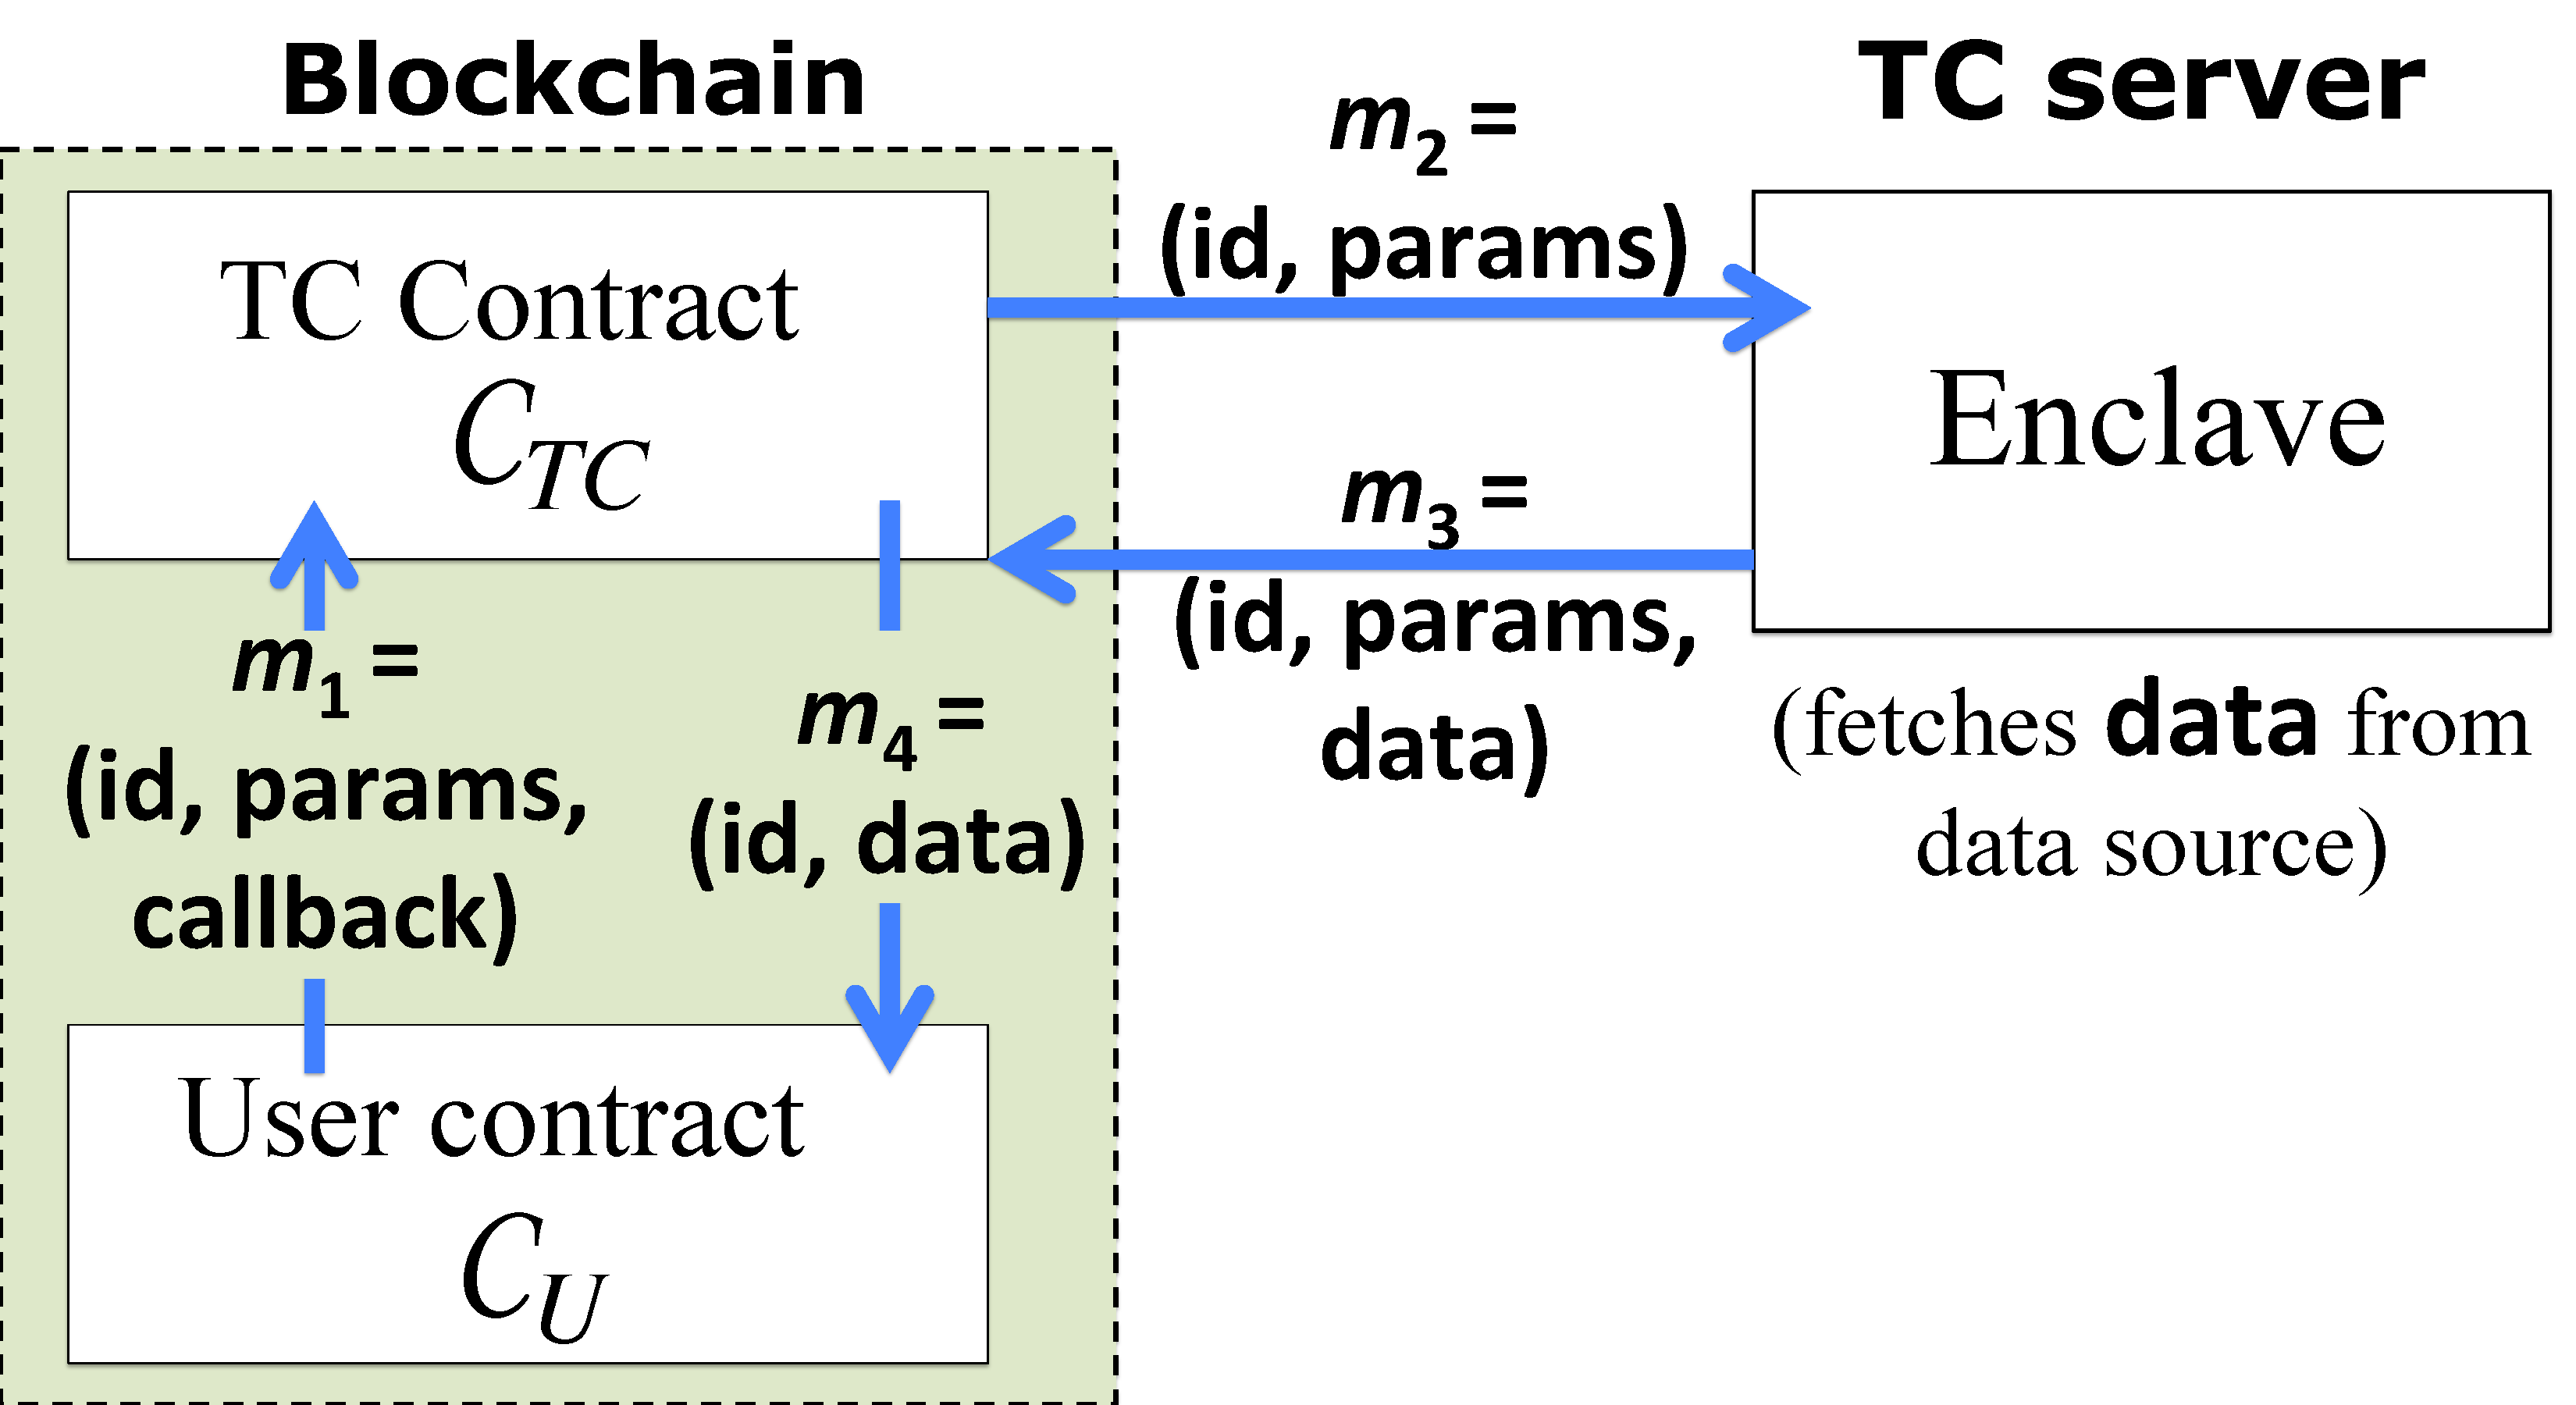
\includegraphics[width=\columnwidth]{figures/DataflowFig}
%\caption{{\bf Data flows in datagram processing.} \elaine{the figure must be changed,
%  m1 and m4 do not have id in the formal algorithm descriptions} }
%\label{fig:dataflow}
%\end{figure}


Digital signatures are needed to authenticate messages, such as $m_3$, entering the blockchain from an external source. We let $(\skTC, \pkTC)$ denote the private / public keypair associated with the \encname for such message authentication. For simplicity, Fig.~\ref{fig:dataflow} assumes that the \encname can send signed messages directly to \tcont. We explain shortly how Ethereum requires a layer of indirection such that \tc sends $m_3$ as a transaction via an Ethereum wallet \tcadd.


\subsection{Use of SGX}
\label{sec:useofsgx}

Let $\enclaveprog$ represent the code for \encname, which we presume is trusted by all system participants. Our protocols in \tc rely on the ability of SGX to attest to execution of an instance of $\enclaveprog$ and bind a public key $\pkTC$ to this instance. Here we briefly explain how we achieve these goals. First, we present a model that abstracts away implementation details in SGX, helping simplify our protocol presentation and later our security proofs. We then explain how SGX attestation is used to authenticate datagrams served by \tcont, namely through binding of $\pkTC$ to an Ethereum wallet on the blockchain. Finally, we explain how we use the clock in SGX. Our discussion draws on formalism for SGX from~\cite{sgxsok}.


%\vspace{-3mm}
\paragraph{\bf Formal model and notation.} 
We adopt a formal abstraction
of Intel SGX proposed by Shi et al.~\cite{sgxsok}. %\elaine{cite}.
Following the UC and GUC paradigms~\cite{uc,guc,juc}, Shi et al.
propose to 
abstract away the details of SGX implementation,
and instead view SGX
as a third party trusted
for both confidentiality and integrity.
Specifically, we use a global UC  
functionality $\fsgx(\sigsgx)[\enclaveprog, \relay]$
to denote (an instance of) an SGX functionality parameterized
by a (group) signature scheme $\sigsgx$.
Here $\enclaveprog$ denotes the SGX enclave program and \relay the physical
SGX host (which we assume for simplicity is the same as that for the \tc~\medname).
As described in Fig.~\ref{fig:SGX_abstraction}, upon initialization, \fsgx runs ${\sf outp} := \enclaveprog.{\bf Initialize}$()
and attests to the code of $\enclaveprog$ as well as ${\sf outp}$.
Upon a resume call with ${(\sf id, params)}$, \fsgx runs and outputs the result of
$\enclaveprog.{\bf Resume}({\sf id, params})$.
Further formalism for \fsgx is given in Appendix~\ref{sec:sgxmodel}.
%Shi et al. \elaine{cite} propose a formal
%abstraction that captures a subset of the features
%of Intel SGX. Their model follows the UC and GUC paradigm~\cite{uc,guc,juc}.
%In this paper, we use the same formal abstraction
%to model SGX (see Figure~\ref{fig:fsgx}).
%\elaine{explain more here, we can think of fsgx as a trusted third party.}

%The main idea behind the UC modeling proposed by Shi et al.
%\elaine{cite}
%
%We abstract away details of the functioning of SGX in two ways.
%First, we abstract away the use of group signatures in EPID and simply denote the keypair associated with group signatures for all legitimate SGX hosts by $(\pkM, \skM)$. 
%We let $\Sigma.{\sf Sign}({\sk}, X)$ denote a digital signature under private key $\sk$ of message $X$, and $\Sigma.{\sf Verify}({\sk}, \sigma, X)$ denote the corresponding verification operation. 
%
%Second, we model execution in SGX in terms of a functionality $\fsgx$ operating in a stateful manner on \enclaveprog \xxx[Fan]{Do we want to provide some intuition such that people with no UC background can still read our protocol correctly? For example, maybe we can briefly explain the difference between functionality and protocol?}, and specified in Figure~\ref{fig:SGX_abstraction}. $\fsgx$ may be be invoked with one of two messages to \enclaveprog : \initcall, which creates the enclave with \enclaveprog as its initial state and triggers measurement quotes, and (\resumecall, $X$) which initiates an execution of \enclaveprog on a fresh input $X$. (We assume that \enclaveprog exits only when it completes processing of a given input.) We let $\fsgx[\enclaveprog, \relay]$ denote invocation of $\fsgx$ on \enclaveprog by \relay. 
%

\begin{figure}[ht!]
\begin{boxedminipage}{\columnwidth}
\begin{center}
{\bf $\fsgx[\enclaveprog, \relay]$: abstraction for SGX}
\end{center}
\begin{tabular}{l}
{\bf{\em Hardcoded}}: $\skM$ \\[3pt]
{\bf {\em Assume}}:
{\small $\enclaveprog$ has entry points {\bf Initialize} and {\bf Resume}}\\[3pt] 

{\bf Initialize:}\\
On receive (\initcall) from $\relay$: \\
\quad Let ${\sf outp} := \enclaveprog.{\bf Initalize}()$  \\
\quad \sgray{\it //~models EPID signature.}\\
\quad $\sigatt := \sigsgx.{\sf Sign}(\skM, (\enclaveprog, {\sf outp}))$\\
\quad Output  $({\sf outp}, \sigatt)$\\[5pt]

{\bf Resume:}\\
On receive (\resumecall, {\sf id}, {\sf params}) from $\relay$: \\
\quad Let ${\sf outp} := \enclaveprog.{\bf Resume}({\sf id, params})$  \\
\quad Output ${\sf outp}$ 
\end{tabular}
\end{boxedminipage}
\caption{Formal abstraction for SGX execution capturing a subset of SGX features
sufficient for implementation of \tc.}
\label{fig:SGX_abstraction}
\label{fig:fsgx}
\end{figure}

%\vspace{-3mm}
\paragraph{Binding $\enclaveprog$ to Ethereum wallet \tcadd.}
Information can only be inserted into the blockchain in Ethereum as a transaction from a wallet. Thus, the only way the \medname can relay messages from the \encname to \tcont is through a wallet \tcadd. Since the \medname may corrupt messages, however, it is critical that they be authenticated by the \encname. Since Ethereum itself 
already verifies signatures on transactions from externally owned accounts (i.e., users interact with the  Ethereum blockchain through an authenticated channel), \tc uses a trick to {\it piggyback verification of enclave signatures on top of Ethereum's already existing transaction signature verification mechanism}. 
Very simply, the \encname creates \tcadd with the public key \pkTC. 

To make this idea work fully, the public key $\pkTC$ must be hardcoded into \tcont. A client creating or relying on a contract that uses \tcont is responsible for making sure that this hardcoded $\pkTC$ has an appropriate SGX attestation before interacting with the $\tcont$  blockchain contract.  Let {\sf Verify} denote a verification algorithm for EPID signatures. Fig.~\ref{fig:att_check} gives the protocol for a client to check that \tcont is backed by a valid \encname instance. (We omit modeling here of IAS online revocation checks.)

%This protocol does not include a mechanism for \emph{revocation} of a compromised SGX instance, an issue we discuss later in the paper.

In summary, then, we may assume in our protocol specifications that {\em relying clients have verified an attestation for \encname and thus that datagram responses sent from \tcadd to \tcont are trusted to originate from \engine.} 



\begin{figure}[htb!]
\begin{boxedminipage}{\columnwidth}
\begin{center}
{\bf User: offline verification of SGX attestation}
\end{center}
\begin{tabular}{l}
{\bf {\em Inputs}}: $\pkM$, $\pkTC$, $\enclaveprog$, $\sigatt$ \\[5pt]
{\bf Verify:} \\
Assert $\enclaveprog$ is the expected enclave code\\
Assert $\sigsgx.{\sf Verify}(\pkM, \sigatt, (\enclaveprog, \pkTC))$ \\
Assert \tcont is correct and parametrized w/ \pkTC\\
\sgray{\it //~now okay to rely on \tcont}
\end{tabular}
\end{boxedminipage}
\caption{A client checks an SGX attestation on the enclave's code $\enclaveprog$ and public key $\pkTC$.
  The client also checks that $\pkTC$ is hardcoded into \tc blockchain contract \tcont before using \tcont.
} 
\label{fig:att_check}
\end{figure}


%\vspace{-3mm}
\paragraph{\bf SGX Clock.}
As noted above, the trusted clock for SGX provides only relative time with respect to a reference point.
To work around this, the \encname is initialized with the current wall-clock time provided by a trusted source, e.g.~the \medname (under a trust-on-first-use model).
In the current implementation of \tc, clients may, in real time, request and verify a fresh timestamp---signed by the \encname under \pkTC---via a web interface in the \medname.
Thus, a client can determine the absolute clock time of the \encname to a degree of accuracy bounded by the round-trip time of its attestation request plus the attestation verification time---hundreds of milliseconds in a wide-area network.
This high degree of accuracy is potentially useful for some applications but only loose accuracy is required for most. Ethereum targets a block interval of 12 s and the clock serves in \tc primarily to: (1) Schedule connections to data sources and (2) To check TLS certificates for expiration when establishing HTTPS connections. For simplicity, we assume in our protocol specifications that the \encname clock provides accurate wall-clock time in the canonical format of seconds since the Unix epoch January 1, 1970 00:00 UTC.

We let $\clock()$ denote measurement of the SGX clock from within the enclave, expressed as the current absolute (wall-clock) time. 


\subsection{A Payment-Free Basic Protocol}
\label{sec:payment-free-protocol}

For simplicity, we first specify a payment-free version of our basic protocol, i.e.~one that does not include gas or fees. Later, in our implementation discussion, we explain how we handle these two resources and we prove payment-related properties in the paper appendix. For simplicity, we assume a single instance of \engine, although our architecture could scale up to multiple enclaves and even server instances. To show messages corresponding to those in Fig.~\ref{fig:dataflow}, we use the label $(\msgi{i})$.

%\vspace{-3mm}
\paragraph{The Requester Contract $\reqcont$.}
The requester contract $\reqcont$ sends to the \tcontract \tcont
a request of the form $(\dgform, \dgcallback)$.
%which \tcont converts into a message $m_1 = (\dgform, \dgcallback)$ as specified below.

%\vspace{-3mm}
\paragraph{The \tcontract \tcont.} 
The \tcontract, as noted above, accepts a datagram request from \reqcont, 
assigns a unique ${\sf id}$ to each request, and
records the request.
%\tcont
%now
%forwards the request to the \tc server, and 
Our Town Crier Relay $\relay$ monitors
requests received by \tcont and 
forwards them to an SGX enclave.
When $\tcont$ obtains a valid response
from $\tcadd$,   
it 
sends the resulting datagram $\dgm$ to the entry point \dgcallback 
specified by the requesting contract \reqcont. As explained above, because the response $(\msgi{2})$ comes from $\tcadd$, the blockchain automatically verifies that the response is correctly signed under $\engine$'s key $\pkTC$ and \tcont need not verify the signature explicitly. \tc does, however, have a subtle security requirement. Specifically,  for a given datagram request $\dgid$, \tcont must verify that $\dgform' = \dgform$, where $\dgform'$ is in the digitally signed message produced by \engine and $\dgform$ is the locally stored parameters. The check is necessary to prevent \relay from corrupting datagram requests passed by \tcont (which, as a public function, has no means of digitally signing requests). 

\tcont is specified in Fig.~\ref{fig:tc-contract}. Here, Call denotes a call to a contact entry point. 

\begin{figure}[!htb]
\begin{tabularx}{\linewidth}{|@{\hspace{3pt}}r@{\hspace{1ex}}X@{\hspace{3pt}}|}
  \hline

  \multicolumn{2}{|c|}{{\bf Program for Town Crier blockchain contract \tcont}} \\ [1ex]

  {\bf Initialize:} &  Counter := 0 \\[1ex]

  {\bf Request:} & On recv $(\dgform, \dgcallback)$ from some $\reqcont$: \\
                 & \dgid :=  Counter; \ \ Counter := Counter + 1 \\
                 & Record $(\dgid, \dgform, \dgcallback)$ \hfill \sgray{\it //~\msgi{1}} \\[1ex]

  {\bf Deliver:} & On recv $(\dgid, \dgform, \dgm)$ from $\tcadd$: \\
                 & Retrieve recorded $(\dgid, \dgform', \dgcallback)$ \\
                 & Assert $\dgform = \dgform'$ \\
                 & Call ${\dgcallback}({\dgm})$ \hfill \sgray{\it //~\msgi{4}} \\

  \hline
\end{tabularx}
\caption{
The Town Crier \tcontract \tcont.
}
\label{fig:tc-contract}
\end{figure}

%\vspace{-3mm}
\paragraph{The \encname \engine.} When initialized through {\bf Initialize}(), \engine ingests the current wall-clock time; by storing this time and setting a clock reference point, it calibrates its absolute clock. It generates an ECDSA keypair $(\pkTC,\skTC)$ (parameterized as in Ethereum), where $\pkTC$ is bound to the \engine instance through insertion into attestations.  

Upon a call to {\bf Resume}$({\sf id}, {\sf params})$, \engine contacts the data source specified by {\sf params} via HTTPS and checks that the corresponding certificate {\sf cert} is valid. (We discuss certificate checking in Appendix~\ref{sec:impl}.) Then \engine fetches the requested datagram and returns it to \relay along with $\dgform$ and $\dgid$, all digitally signed with $\skTC$.  Fig.~\ref{fig:engineprotocol} shows the protocol for \engine.

\begin{figure}[!h]
\begin{boxedminipage}{\columnwidth}
\begin{center}
{\bf Program for \tcs~\encname ($\enclaveprog$)}
\end{center}
\begin{tabular}{l} 
{\bf Initialize}\,$({\sf void})$ \\ %{\it //~called only once upfront}\\
%\quad Set clock reference point\\
%\quad Record $T_0$ \elaine{this is never used} \\ 
%\elaine{i deleted the clock implementation, we can separate abstraction from implementation.}\\
\quad \sgray{\it// Subroutine call from $\fsgx$, which attests to}\\ 
\quad \sgray{\it// $\enclaveprog$ and $\pkTC$. See Figure~\ref{fig:SGX_abstraction}.} \\
\quad $(\pkTC, \skTC) := \Sigma.{\sf KeyGen}(1^\lambda)$\\
%\quad Record $(\pkTC, \skTC)$\\
\quad Output $\pkTC$   \\[3pt]

%{\bf Attest}:  On recv \attcall: \\ %{\it //~called only once upfront}\\
%\quad $T := \clock()$\\
%\quad Call quoting enclave with supp.~data $(\pkTC, T)$
%\\[5pt]

{\bf Resume}\,$(\dgid, \dgform)$\\
\quad Parse ${\sf params}$ as $(\weburl, \dgspec, T) $:\\
\quad Assert $\clock() \geq T.{\sf min}$\\
\quad Contact $\weburl$ via HTTPS, obtaining ${\sf cert}$ \\
\quad Verify {\sf cert} is valid for time $\clock()$\\
\quad Obtain webpage $w$ from $\weburl$ \\
\quad Assert $\clock() \leq T.{\sf max}$\\
\quad Parse $w$ to extract \dgm with specification \dgspec \\
\quad $\sigma := \Sigma.{\sf Sign}({\skTC}, ({\sf id}, {\sf params}, {\sf data}))$\\
\quad Output $(({\sf id}, {\sf params}, {\sf data}), \sigma)$
\end{tabular}
\end{boxedminipage}
\caption{
The \tcs~\encname \engine.
} 
\label{fig:engineprotocol}
\end{figure}

%\vspace{-3mm}
\paragraph{The \medname \relay.}
As noted in Section~\ref{sec:architecture},
\relay bridges the gap between the \encname and the blockchain in three ways.
(1) It scrapes the blockchain and monitors \tcont for new requests $(\dgid, \dgform)$.
(2) It boots the \encname with \engine.{\bf Initialize}() and calls \engine.{\bf Resume}$(\dgid, \dgform)$ on incoming requests.
(3) it forwards datagram responses from \engine to the blockchain.
Recall that it forwards already-signed transacations to the blockchain as \tcadd.
%Recall that it sends transactions to the blockchain and thus forwards responses as \tcadd.
The program for \relay is shown in Fig.~\ref{fig:relayprotocol}.
The function {\sf AuthSend} inserts a transaction to blockchain (``as $\tcadd$'' means the transaction is already signed with $\skTC$).
An honest \medname will invoke \engine.{\bf Resume} exactly once with the parameters of each valid request and never otherwise.

\begin{figure}[h!]
\begin{tabularx}{\linewidth}{|@{\hspace{3pt}}p{1em}@{\hspace{1ex}}X@{\hspace{3pt}}|}
  \hline

  \multicolumn{2}{|c|}{\bf Program for Town Crier \medname $\relay$} \\[1ex]

  \multicolumn{2}{|l|}{\bf Initialize:} \\
                    & Send \initcall to $\fsgx[\enclaveprog, \relay]$ \\
                    & On recv $(\pkTC, \sigatt)$ from $\fsgx[\enclaveprog, \relay]$: \\
                    & \quad Publish $(\pkTC, \sigatt)$ \\[1ex]

  \multicolumn{2}{|l|}{{\bf Handle}$(\dgid, \dgform)$:} \\
                    & Parse \dgform as $(\_, \_, T)$ \\
                    & Wait until ${\sf clock}() \geq T.{\sf min}$ \\
                    & Send $(\text{\resumecall}, \dgid, \dgform)$ to $\fsgx[\enclaveprog, \relay]$ \\
                    & On recv $((\dgid, \dgform, \dgm), \sigma)$ from \\ & $\fsgx[\enclaveprog, \relay]$: \\
                    & \quad  {\sf AuthSend} $(\dgid, \dgform, \dgm)$ to \tcont as \tcadd \\
                    & \quad \sgray{\it //~send out $\msgi{3}$} \\[1ex]

  \multicolumn{2}{|l|}{\bf Main:} \\
                    & Loop Forever: \\
                    & \quad Wait for \tcont to records request $(\dgid, \dgform, \_)$: \\
                    & \quad Fork a process of {\bf Handle}$(\dgid, \dgform)$ \\
                    & End \\

  \hline
\end{tabularx}
\caption{The Town Crier \medname \relay.}
\label{fig:relayprotocol}
\end{figure}


